\chapter{Anforderungen}
\section{Benutzer und Personas}
Die Benutzer der Project Helin Plattform teilen sich in drei Gruppen auf.
\begin{itemize}
	\item{\textbf{Kunde:} Der Kunde möchte Produkte und Dienstleistungen nutzen, welche von Drohnen erbracht werden können. Beispielsweise die Bestellung eines Getränks und sofortige Lieferung an seine Position.}
	\item{\textbf{Administrator:} Administratoren verwenden die Project Helin Plattform um eine Flotte von Drohnen zu verwalten. Sie nutzen dazu die Webseite der Plattform und definieren, wo ihre Drohnen fliegen dürfen und welche Produkte und Services wo angeboten werden.}
	\item{\textbf{Drone-Operator:} Der Drone-Operator ist für die Wartung der Drohne verantwortlich und verwendet dafür die Onboard-App. Er kümmert sich ausserdem um die Beladung der Drohnen.}
\end{itemize}

Bei den Personas handelt es sich um fiktive Personen.
\subsection{Persona Diego: Kunde}
\begin{minipage}{0.25\textwidth}% adapt widths of minipages to your needs
\centering
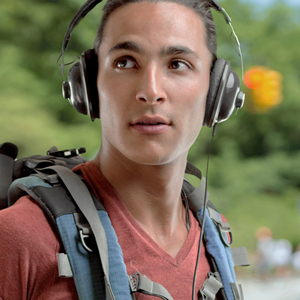
\includegraphics[width=1.0\textwidth]{images/persona-diego.jpg}
\captionof{figure}{Diego\protect\footnotemark[1]}
\label{fig:diego}
\end{minipage}%
\hfill%
\begin{minipage}{0.70\textwidth}
Diego ist \textbf{23 Jahre alt} und wohnt in einer WG in Uster.
Diego hat eine Informatik-Lehre mit BMS abgeschlossen und ist auf der Suche nach einer neuen beruflichen oder schulischen Herausforderung.
\paragraph{Technisches Verhalten}
Er arbeitet täglich acht Stunden mit dem PC und nutzt gerne neue Technologien. Er besitzt ein Android-Smartphone der neusten Generation. Die Android Updates macht er immer sofort. Interessiert sich für neue Technologien und sieht sich regelmässig Kickstarter Projekte an.
\paragraph{Ziele}
Er will sich weiterbilden und neue Herausforderungen finden. Er möchte neue Technologien entdecken und einsetzen.
\end{minipage}

\footnotetext[1]{ Freie Lizenz, \protect\url{Quelle: http://blog.placeit.net/free-avatar-pack/}}
\newpage

\subsection{Persona Stefanie: Administrator}
\begin{minipage}{0.25\textwidth}% adapt widths of minipages to your needs
\centering
	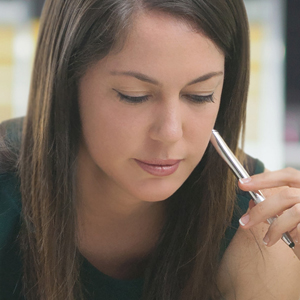
\includegraphics[width=1\textwidth]{images/persona-stefanie.jpg}
	\captionof{figure}{Stefanie \protect\footnotemark[1]}
	\label{fig:stefanie}
\end{minipage}
\hfill %
\begin{minipage}{0.70\textwidth}
Stefanie ist \textbf{33 Jahre alt} und lebt alleine in Zürich.

Stefanie arbeitet bei einer Eventagentur und hat eine Ausbildung als Eventmanagerin abgeschlossen.

\paragraph{Technisches Verhalten}
Sie nutzt den PC täglich 8 Stunden bei der Arbeit, vor allem Excel, Word und das E-Mail-Programm. Ausserdem hat sie viel Erfahrung mit diversen mandantenfähigen Systemen (CRM, ERP), die als Web-Applikationen umgesetzt sind. Sie nutzt Chrome als Browser während der Arbeit. Sie besitzt ein Samsung Galaxy S4, dass sie schon seit einigen Jahren verwendet.
\paragraph{Kommunikationsverhalten}
Sie kommuniziert geschäftlich hauptsächlich per E-Mail. Mit Freunden unterhält sie sich oft über WhatsApp oder den Facebook-Messenger. Sie surft öfters während der Arbeit auf Facebook.
\paragraph{Ziele}
Sie möchte mit neuen und innovativen Ideen Events für Besucher spannender gestalten.
\end{minipage}

\subsection{Persona Ricardo: Drone Operator}
\begin{minipage}{0.25\textwidth}
\centering
	
\includegraphics[width=1\textwidth]{images/persona-ricardo.jpg}
	\captionof{figure}{Ricardo \protect\footnotemark[1]}
	\label{fig:ricardo}
\end{minipage}
\hfill %
\begin{minipage}{0.70\textwidth}
Ricardo ist \textbf{26 Jahre} alt und wohnhaft in Wetzikon. Der ausgebildete Schlosser hat zur Zeit keinen festen Job. Er lebt das Leben von Tag zu Tag und geniesst, es keine festen Verpflichtungen zu haben.
\paragraph{Technisches Verhalten}
Er nutzt den PC selten, vorallem aber zum Surfen im Internet. Als Mobiltelefon besitzt er ein altes Telefon mit Android. Er möchte sich auch kein neues Gerät kaufen, da er ausser WhatsApp und der Taschenlampe das Gerät sowieso nicht verwendet.
\paragraph{Kommunikationsverhalten}
Er verwendet hauptsächlich sein Mobiltelefon zur Kommunikation. Mit Freunden ist er über WhatsApp in Kontakt.
\paragraph{Ziele}
Ricardo möchte gerne am mit kleinen Jobs etwas Geld dazu verdienen und ohne grosse Einarbeitungszeit den Anforderungen der Eventtechnikfirma genügen.
\end{minipage}

\footnotetext[1]{ Freie Lizenz, \protect\url{Quelle: http://blog.placeit.net/free-avatar-pack/}}
\section{Szenario}

Um eine bessere Übersicht über die Anforderungen zu erhalten wurde folgendes Szenario erstellt. Die rechtliche Situation wird dabei ausser Acht gelassen:\\

\textbf{Stefanie} hat in einem Facebook-Post von Project Helin erfahren und möchte deshalb am nächsten Openair, das ihre Firma organisiert, einen Getränke-Lieferservice mit Drohnen anbieten. Sie registriert sich und ihre Organisation auf \url{https://my.helin.ch/} und lässt sich von einem lokalen Anbieter zwei Drohnen bauen, die die Getränke tragen und abwerfen können. Nach dem Aufbau des Festgeländes zeichnet sie die Flugzonen auf \url{https://my.helin.ch/} auf der Karte ein. Sie engagiert ausserdem Ricardo, der die Drohnen beladen und warten soll. Dieser lädt ein App herunter und installiert sie auf den zwei Smartphones, die auf den Drohnen montiert werden. Um die Drohnen mit dem Server zu verbinden, kann er die Adresse des Servers und einen Code eingeben, den Stefanie auf der Webseite abgeschrieben hat.\\

\textbf{Diego} möchte an einem Openair ein kühles Getränk für sich bestellen. Er hat auf einem Plakat vor Ort gesehen, dass ein Drohnen-Lieferservice existiert. Er lädt die Project Helin Bestell-App herunter und bestellt ein Rivella. Ihm wird eine Karte angezeigt mit dem voraussichtlichen Lieferort, den er bestätigen muss. Er muss sich nun einloggen und die Ware auf dem Mobiltelefon mit seiner Kreditkarte bezahlen.\\

\textbf{Ricardo} erhält eine Nachricht auf dem Onboard-App, die ihn fragt ob die Drohne einsatzbereit ist. Er bestätigt und ihm wird angezeigt, dass er ein Rivella laden muss. Er lädt die Flasche zusammen mit dem Fallschirm an die Drohne und bestätigt die Beladung. Die Drohne zeigt einen Countdown an und fliegt nach 10 Sekunden los. \\

\textbf{Diego} wundert sich ob seine Bestellung unterwegs ist und sieht auf einer Karte in der App wie sich die Drohne auf ihn zubewegt. Die Drohne fliegt über ihn und wirft die Ladung ab. Danach fliegt sie auf dem gleichen Weg wieder zurück.\\

\textbf{Ricardo} sieht, dass die Drohne im Anflug ist. Sie landet an der Position, die ihm Stefanie zuvor gezeigt hatte. Er kann nun prüfen ob die Batterie noch genug Spannung hat und ob mit der Drohne sonst alles in Ordnung ist.\\

\textbf{Stefanie} sitzt Zuhause und hat den Flug der Drohne auf \url{https://my.helin.ch/} verfolgt. Sie sieht wie sich der Stand der Batterie während des Flugs geändert hat und das Ricardo gerade eine Drohne deaktiviert hat, bei der er die Batterie tauschen muss.

\newpage
\section{Funktionale Anforderungen (User Stories)}

Die funktionalen Anforderungen leiten sich aus der Aufgabenstellung, sowie den mit dem Betreuer diskutierten Ideen ab. Standardoperationen sind mit Teilen von \Gls{CRUD} bezeichnet. Einige Anforderungen sind mit 'zusätzlich' oder 'ausgeschlossen' gekennzeichnet. Eine Erklärung zu jeder geänderten Anforderung findet sich im nächsten Abschnitt.

\subsection{Administrator}
\begin{itemize}
\item Als Administrator möchte ich auf der Webseite einen Account erstellen können.
\item Als Administrator möchte ich meine Organisation verwalten können (CRU). (zusätzlich, siehe unten)
\item Als Administrator möchte ich neue Administratoren hinzufügen und entfernen können. (zusätzlich)
\item Als Administrator möchte ich ein Projekt erfassen können.
\item Als Administrator möchte ich auf eine Drohne dem Projekt hinzufügen können.
\item Als Administrator möchte ich alle Drohnen verwalten können (RUD).
\item Als Administrator möchte ich Produkte verwalten können (CRUD).
\item Als Administrator möchte ich Produkte einem Projekt hinzufügen können (zusätzlich)
\item Als Administrator möchte ich Services (zum Beispiel Drone Selfies) verwalten können (CRUD). (optional)
\item Als Administrator möchte ich Flug-, Lade- und Abwurfzonen verwalten können (CRUD).
\item Als Administrator möchte ich Bestellungen verwalten können (CRUD) (teilweise ausgeschlossen).
\item Als Administrator möchte ich Telemetriedaten der Drohne, sowie die berechnete Route vor, nach, und während der Auslieferung einer Bestellung ansehen können.
\item Als Administrator möchte ich Bestellungen abbrechen können. (ausgeschlossen)
\end{itemize}

\subsection{Kunde}
\begin{itemize}
	\item Als Kunde möchte ich eine App aus dem Google Play Store herunterladen können um diese verwenden zu können.
	\item Als Kunde möchte ich die App nutzen, ohne mich anmelden zu müssen.
	\item Als Kunde möchte ich in der App, aus einer Liste von Produkten und Services, eine Auswahl treffen können.
	\item Als Kunde möchte ich nur Produkte und Services sehen, die in meiner Umgebung angeboten werden. (zusätzlich)
	\item Als Kunde möchte ich eine Bestellung tätigen können.
	\item Als Kunde möchte ich die bestellte Ware direkt bezahlen können. (optional)
	\item Als Kunde möchte ich auf der Karte des Smartphones die Bewegung der Drohne verfolgen können um abzuschätzen wann meine Lieferung eintrifft.
	\item Als Kunde möchte ich eine Bestellung stornieren können (ausgeschlossen).
\end{itemize}

\subsection{Drone-Operator}
\begin{itemize}
	\item Als Drone-Operator möchte ich eine Android-App mit Hilfe der heruntergeladenen \Gls{APK} installieren können.
	\item Als Drone-Operator muss ich die Drohne beim Server registrieren können.
	\item Als Drone-Operator muss ich die Drohne zu einer Organisation hinzufügen können.
	\item Als Drone-Operator muss ich das \Gls{OTG}-fähige Smartphone an einen \Gls{MAVLink} kompatiblen \Gls{Flight-Controller} über USB anschliessen können.
	\item Als Drone-Operator muss ich eine Verbindung zwischen App und Server über das Internet herstellen könnnen.
	\item Als Drone-Operator muss ich eine Verbindung zwischen App und \Gls{Flight-Controller} herstellen können.
	\item Als Drone-Operator möchte ich den aktuellen Zustand der Verbindungen zur Drohne und zum Server sehen.
	\item Als Drone-Operator möchte ich den aktuellen Status des \Gls{Flight-Controller}s, beispielsweise GPS und Batteriespannung, sehen.
	\item Als Drone-Operator möchte ich eine Liste von Produkten angezeigt bekommen, die für die aktuelle Mission geladen werden müssen.
	\item Als Drone-Operator möchte ich eine Mission annehmen oder ablehnen können, um eine Drohne bei Problemen austauschen zu können.
	\item Als Drone-Operator möchte ich die Beladung einer Drohne bestätigen können.
	\item Als Drone-Operator erhalte ich ein visuelles und akustisches Countdown-Signal bevor die Drohne startet.
	\item Als Drone-Operator möchte ich den Start der Drohne während des Countdowns verhindern können.
\end{itemize}

\subsection{Nachträglich ausgeschlossene Anforderungen}

\subsubsection{Bestellung löschen und ändern}
Gemäss den anfänglichen Anforderungen sollte der Administrator die Möglichkeit haben eine Bestellung zu bearbeiten (\Gls{CRUD}). Dies wurde reduziert auf das Ansehen von Bestellungen (R). Unserer Meinung nach, sollten nur der Kunde die Möglichkeit haben seine Bestellung zu löschen. Ausserdem muss es auch dort Einschränkungen geben, da eine bezahlte Bestellung unter keinen Umständen gelöscht werden darf.

\subsubsection{Mission abbrechen}

Das Abbrechen einer Mission wurde aus dem Scope entfernt, da sich einerseits Fragen über den sinvollen Einsatz eines solchen Features stellten und dafür andere Tasks wie die Bezahlung im App priorisiert werden konnten.

\subsection{Nachträglich hinzugefügte Anforderungen}

\subsubsection{Verwalten von Organisationen}

Um die Applikation mandantenfähig zu machen, wurden Organisationen eingefügt. Diese trennen verschiedene Kunden komplett ab und ermöglichen den Einsatz als Software as a Service.

\subsubsection{Administratoren hinzufügen und entfernen}

Um Organisationen nutzbar zu machen, musste es auch möglich sein, zusätzliche Administratoren zu einer Firma hinzuzufügen und wieder zu entfernen.

\subsubsection{Produkte einem Projekt hinzufügen}

Dieses Feature war nötig, damit Organisationen ihre Produkte nur einmal erfassen müssen und diese dann für verschiedene Projekte (z.B. Events) verwendet werden können (siehe Abb. \ref{fig:domain-model}).

\subsubsection{Nur verfügbare Produkte anzeigen}

Es macht keinen Sinn, dass ein Kunde Produkte sieht, die gar nicht zu ihm geliefert werden können. Deshalb wird die Liste mit Hilfe seiner Position auf verfügbare Produkte gefiltert.

\newpage
\section{Nichtfunktionale Anforderungen}

\subsection{Android Kompatibilität}
\begin{tabular}{|p{.25\textwidth}|p{.75\textwidth}|} \hline
	Synopsis & Die Onboard-App funktioniert mit Android 4.4 und die Customer-App mit Android 6.1\\ \hline
	Messbarkeit & Die obengenannten Apps können alle funktionalen Anforderungen erfüllen, wenn sie mit Android 4.4 bzw. 6.1 gestartet werden.\\ \hline
\end{tabular}

\subsection{Verbindungsabbruch}
\begin{tabular}{|p{.25\textwidth}|p{.75\textwidth}|} \hline
	Synopsis & Verbindungsabbruch der Onboard App zum Server soll keine negativen Auswirkungen auf die Mission haben.  \\ \hline
		
	Messbarkeit & Nach dem Start der Mission schliesst die Drohne, auch ohne Verbindung zum Server, die Mission ab. \\ \hline
\end{tabular}

\subsection{Physische Sicherheit der Drohne}
\begin{tabular}{|p{.25\textwidth}|p{.75\textwidth}|} \hline
	Synopsis & Eine Drohne führt vor dem Freigeben der Motoren (Arming) einen Check durch, der prüft ob alle nötigen Voraussetzungen für einen Start erfüllt sind. Ausserdem müssen vor einem Start ebenfalls Voraussetzungen der Mission erfüllt sein, beispielsweise muss der Drone-Operator den Start freigeben. Sollte eine dieser Vorraussetzungen nicht erfüllt sein, darf die Drohne nicht starten.  \\ \hline
	
	Messbarkeit & Drohne startet nicht, falls der Pre-Flight-Check des Autopiloten nicht erfolgreich war oder Voraussetzungen für die aktuelle Mission nicht erfüllt sind. \\ \hline
\end{tabular}
\subsection{Verbindungswiederherstellung}
\begin{tabular}{|p{.25\textwidth}|p{.75\textwidth}|} \hline
	Synopsis & Nach einem Verbindungsabbruch zwischen dem Server und der Onboard App soll die Verbindung wiederhergestellt werden sobald wieder Internet verfügbar ist. \\ \hline
	
	Messbarkeit & Die Verbindung zwischen Server und App wird nach dem deaktivieren und wieder aktivieren der Internetverbindung(4G) innert 30 Sekunden wiederhergestellt.\\ \hline
\end{tabular}

\subsection{Security}
\subsubsection{Sichere Messaging-Verbindungen}
\label{sec:message-security}
\begin{tabular}{|p{.25\textwidth}|p{.75\textwidth}|} \hline
	Synopsis & Es darf nicht möglich sein, dass jemand die Steuerung einer beim Server registrierten Drohne übernehmen kann.\\ \hline
	Messbarkeit & Der Übertragungskanal vom Server zur Drohne ist verschlüsselt und es können sich keine weiteren \Gls{Message-Producer} anmelden.\\ \hline
\end{tabular}

\subsubsection{Sichere HTTP-Verbindungen}
\begin{tabular}{|p{.25\textwidth}|p{.75\textwidth}|} \hline
	Synopsis & Neben der Messaging Verbindung muss auch die HTTP-Verbindung gesichert sein.\\ \hline
	Messbarkeit & Die Verbindung über den Webbrowser lässt nur HTTPS zu. Die Verbindung vom Customer-App zum Server läuft über HTTPS und Secure-WebSockets. Die Verbindung vom Onboard-App zum Server läuft über HTTPS.\\ \hline
\end{tabular}

\section{Usability und Accessability}

Usability-Tests und Anforderungen in der Accessability wurden bewusst und in Absprache mit dem Betreuer aus dem Scope ausgeschlossen.

\section{Domain-Model}
Aus den funktionalen Anforderungen ergibt sich das folgende Domainmodel.
\begin{landscape}
\begin{figure}[h]
	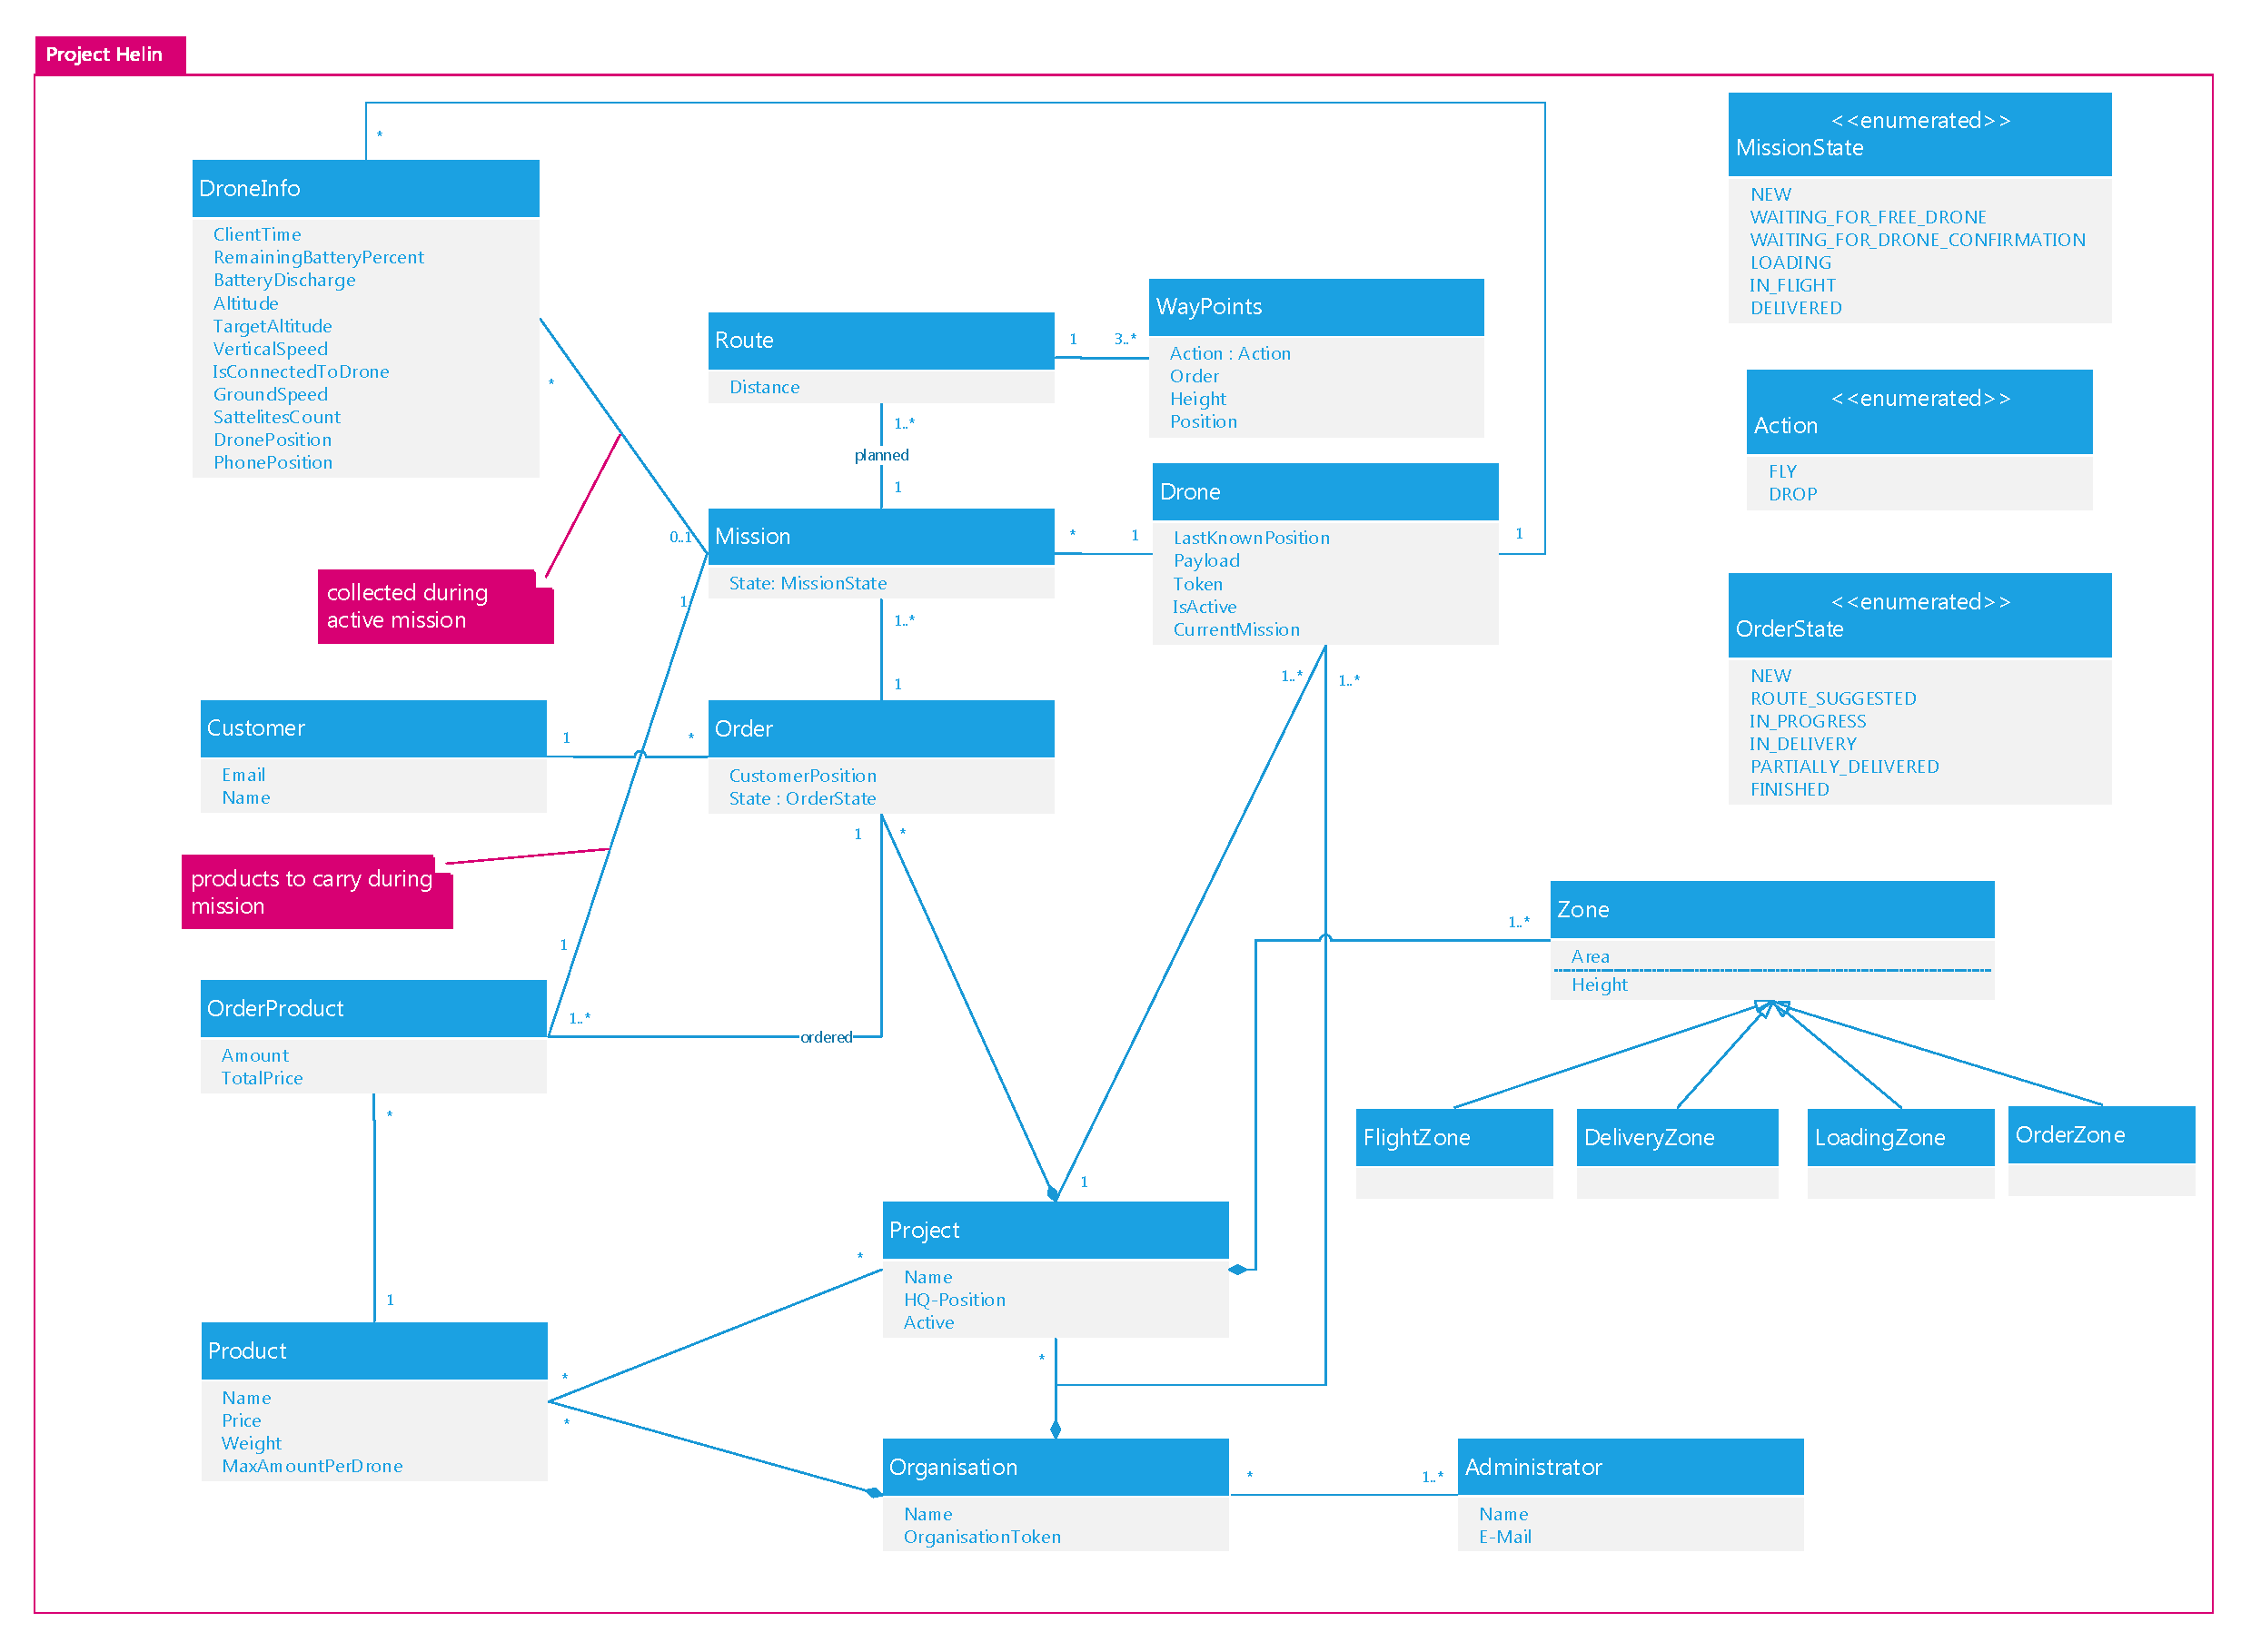
\includegraphics[width=0.75\paperheight]{images/domainmodell.pdf}
	\caption{Domain-Model}
	\label{fig:domain-model}
\end{figure}
\end{landscape}

